\begin{appendices}
    
\chapter{Flutter}
E' impossibile parlare di Flutter senza prima discutere del linguaggio su cui si basa: Dart.\\
Faremo quindi un'introduzione quanto più sintetica possibile sulle sue caratteristiche più proprietarie, tralasciando invece le similitudini a linguaggi popolari che possono facilmente essere intuite dal lettore.
\section{Dart}
Dart è un linguaggio compilato fortemente tipizzato con sintassi simile a C, e adotta molte funzionalità tipiche dei linguaggi moderni: considera infatti ogni variabile un oggetto e implementa la \textit{null safety}, obbligando il programmatore a esplicitare con sintassi specifiche la presenza o meno del valore \verb+null+.

\begin{lstlisting}[language=dart, firstnumber=1,caption={Dart \textit{null safety}}]
//dichiarazione di variabili
String variabileNotNullable = '';  //non puo' mai essere null
String? variabileNullable = null;  //puo' anche essere null

//utilizzo esplicito di variabile nullable
fun (variableNullable);   //compile error
fun (?variableNullable);  //esplicito che puo' essere nulla

//utilizzo esplicito di variabile not nullable
if (value != null)
    fun (!value);   //dico al compilatore che sono certo value != null
\end{lstlisting} 

Permette inoltre l'interpolazione di stringhe:

\begin{lstlisting}[language=dart, firstnumber=1,caption={Dart interpolazone stringhe}]
//sfrutto il simbolo $
'number = $variableName';              //inserisco in stringa 
                                       //direttamente una variabile
'expressionResult = ${expression}';    //inserisco in stringa
                                       //direttamente un'espressione
\end{lstlisting}

Dart tratta in maniera particolare le funzioni, che sono oggetti, hanno un tipo (\verb+Function+), possono avere parametri posizioni o nominali, obbligatori od opzionali: 

\begin{lstlisting}[language=dart, firstnumber=1,caption={Dart parametri funzioni}]
//parametri obbligatori posizionali
void fun (int a, int b);  //non possono essere nulli

//possono essere anteceduti da parametri posizionali opzionali
void fun (int a, int b, [String opz1 = '', String opz2 = '']){}
void fun (int a, int b, [String? opz1nullable, String? opz2nullable]){}

//oppure possono essere anteceduti da parametri nominali opzionali
void fun (int a, int b, {String opz1 = '', String opz2 = ''}){}
void fun (int a, int b, {String? opz1nullable, String? opz2nullable}){}

//non possono essere anteceduti da entrambi
//il seguente codice non compila:
void fun (int a, int b, [String opz1 = ''], {String opz2 = ''}){} 

//tutti i costruttori in Dart hanno solo parametri nominali
//di default i parametri nominali sono opzionali
//possono pero' essere resi obbligatori con la keyword 'required'
void fun ({required String obb1, 
           required String? obb2, 
           String opz1 = ''}){}
\end{lstlisting}

Esistono le funzioni anonime (largamente sfruttate nei metodi \verb+build+ di Flutter), che possono essere ovviamente passate come argomento ad altre funzioni, essendo oggetti:

\begin{lstlisting}[language=dart, firstnumber=1,caption={Dart funzioni anonime}]
//prima sintassi
(){
    //corpo della funzione anonima
} 

//seconda sintassi
() => return_expression

//assegnamento di funzione anonima ad una variabile
//ritorna una stringa con un messaggio portato in upper case
var upperfy = (msg) => '${msg.toUpperCase()}';

//passaggio di funzione come parametro
fun (firstValue, () => secondValue);
\end{lstlisting}

Abbiamo delle espressioni condizionali specifiche del linguaggio dalla grande espressività e che quindi vengono largamente usate:

\begin{lstlisting}[language=dart, firstnumber=1,caption={Dart espressioni ternarie}]
//primo tipo di condizione, detta ternaria
condizione ? expr1 : expr2;

//equivale a (in pseudocodice):
if (condizione == true) return expr1
else                    return expr2

//vediamo un esempio
int? a;               //a==null di default
a = a==null ? 1 : 0;  //ad 'a' viene assegnato il valore 1 
                      //siccome a==null


//################################
//secondo tipo di condizione peculiare:
expr1 ?? expr2;

//equivale a (in pseudocodice):
if (expr1 != null) return expr1
else               return expr2

//vediamo un esempio
int? a;      //a==null di default
a = a ?? 1;  //ad 'a' viene assegnato il valore 1 siccome a==null
\end{lstlisting}

I caratteri \verb+?+ e \verb+!+ sono, come si evince dalle espressioni ternarie e dalla \textit{null safety}, di cruciale importanza in Dart, ed è quindi opportuno vederne ancora qualche esempio:

\begin{lstlisting}[language=dart, firstnumber=1,caption={Dart operatori '?' e '!'}]
list[1]     //accede al secondo elemento della lista

list.?[1]
//equivale a (in pseudocodice):
if (list[1] != null)    return list[1]
else                    return null

//##############################

foo?.bar 
//equivale a (in pseudocodice):
if (foo.bar != null)    return foo.bar
else                    return null

//##############################

foo!.bar
//equivale a (in pseudocodice):
if (foo.bar != null)    return foo.bar
else                    throw (runtimeException)
\end{lstlisting}

Le applicazioni \textit{mobile} e \textit{web} spesso si trovano a eseguire istruzioni che richiedono l'attesa di risorse esterne (ottenere dati dalla rete o leggerli da un \textit{file}, oppure scrivere su un \textit{database}). Per evitare il completo blocco dell'esecuzione (disastroso per un applicativo \textit{consumer}) Dart implementa nativamente delle funzioni di programmazione asincrona, che permetto di svolgere operazioni anche mentre altre sono in attesa.\\
Per fare ciò si serve di tre \textit{keyword}: \verb+async+, \verb+await+ e \verb+Future+:

\begin{lstlisting}[language=dart, firstnumber=1,caption={Dart programmazione asincrona}]
Future<void> checkVersion () async {
    var version = await lookUpVersion();
}

//un'espressione marcata con la keyword 'await' ritorna sempre Future<T>
\end{lstlisting}

Trattiamo infine le caratteristiche peculiari di Dart per quanto riguarda classi e metodi:

\begin{itemize}
    \item Esistono i costruttori costanti, marcati \verb+const+, che sono inizializzati a \textit{compile-time}. Tutti gli altri sono implicitamente dinamici (quindi \textit{run-time});
    \item Posso creare costruttori nominati per implementare costruttori multipli tramite la sintassi:
\begin{lstlisting}[language=dart]
ClassName.constructorName () :
    firstField = firstValue,
    secondField = secondValue;
\end{lstlisting}
    \item Ogni entità è una classe, ogni classe discende da \verb+Object+ (a eccezione di \verb+Null+);
    \item Per ogni classe viene creata un'interfaccia implicita che contiene tutti i membri d' istanza della classe;
    \item I metodi \textit{getter} e \textit{setter} di una classe vengono creati implicitamente per variabili non \verb+final+, ma possono essere definiti esplicitamente con le \textit{keyword} \verb+get+ e \verb+set+.
\end{itemize}

\section{Widget}
Mostriamo ora alcuni componenti di Flutter necessari al proseguimento della lettura, partendo dai \textit{widget}: riprendono l'idea di React di costruire tutta l'interfaccia grafica tramite uno \textit{stack} di \textit{widget}, che definiscono il proprio aspetto basandosi sulla configurazione e lo stato attuali. Quando lo stato di un \textit{widget} cambia, esso riscrive la propria descrizione (insieme di istruzioni e valori che lo determinano) e il \textit{framework} valuta le differenze tra questa e la descrizione precedente per apportare le modifiche necessarie al suo \textit{render tree} e quindi, ultimamente, modificarne l'aspetto e finalizzare il cambio di stato.

\begin{figure}[H]
    \centering
    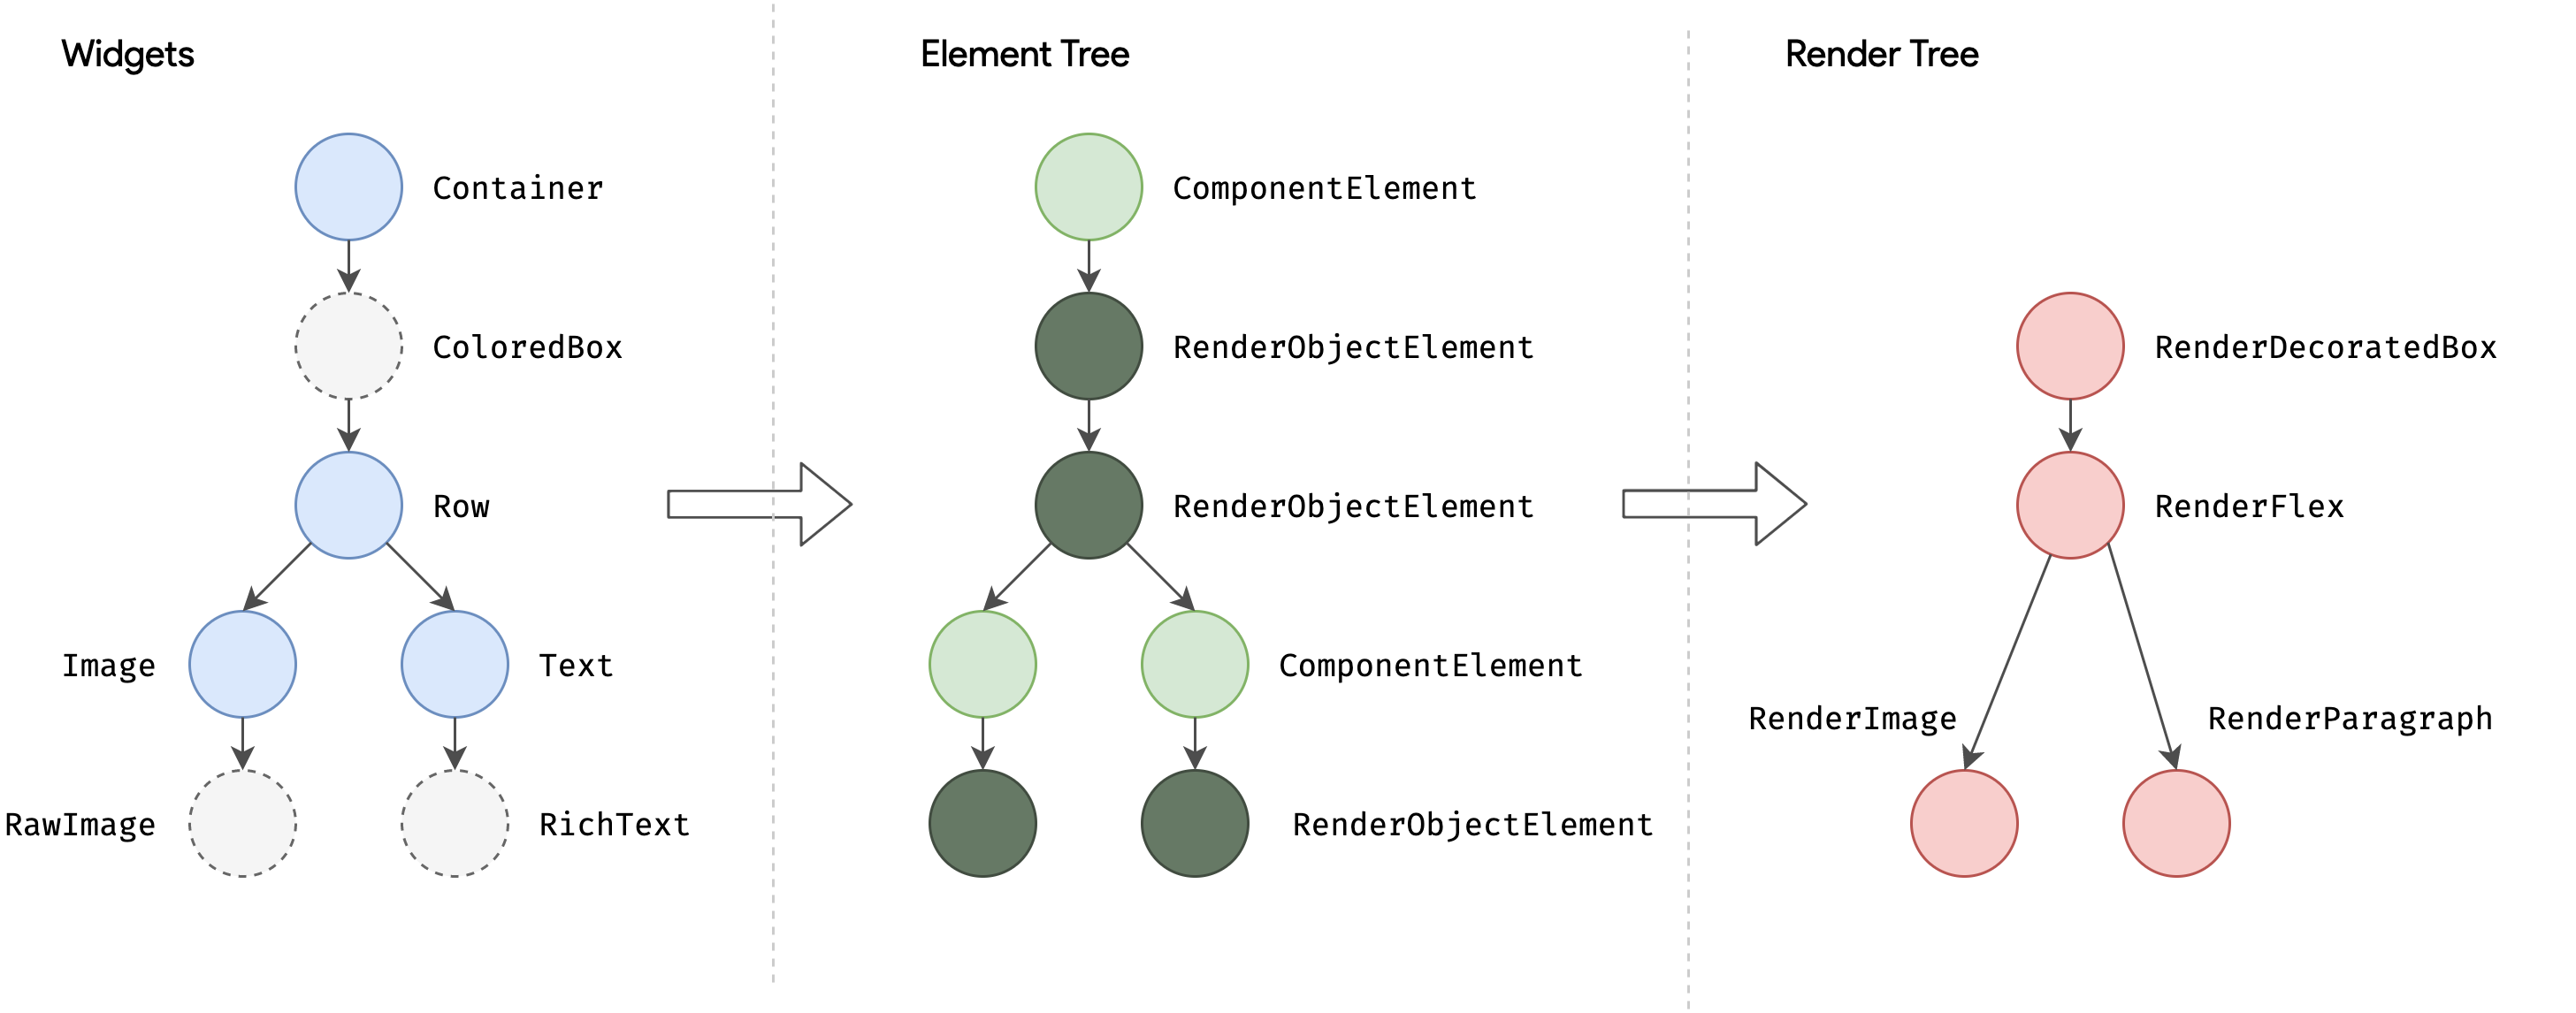
\includegraphics[width=\textwidth]{Flutter_trees}
    \caption[I tre alberi di Flutter]{Flutter usa tre alberi logici come rappresentazione delle proprie strutture: uno per i \textit{widget}, uno per gli \textit{element} e infine quello di \textit{render}.\footnotemark}
    \label{fig:flutter-trees}
\end{figure}
\footnotetext{Fonte: \url{https://docs.flutter.dev/resources/architectural-overview}}

L'albero di \textit{render} è una delle tre strutture logiche che Flutter usa per descrivere i propri oggetti e le proprie interfacce grafiche: \textit{widget tree}, \textit{element tree} e \textit{render tree}. \\
Il \textit{widget tree} rappresenta gli elementi di un \textit{widget} come uno \textit{stack} di \textit{widget}, messi in relazione con il loro elemento padre e i loro elementi figli. Quello mostrato in figura \ref{fig:flutter-trees}, ad esempio, rappresenta un \verb+Containter+ che contiene un \verb+ColoredBox+ che a sua volta contiene una \verb+Row+ e via dicendo. I \textit{widget} sono per definizione immutabili, quindi una modifica richiede necessariamente una distruzione e successiva ricreazione del \textit{widget} interessato.\\
Vediamo un esempio più specifico di \textit{widget tree}:

\begin{lstlisting}[language=dart, caption={Codice rilevante per la parte grafica dell'\textit{app} di esempio di Flutter}]
Widget build(BuildContext context) {
    return Scaffold(
      appBar: AppBar(
        title: Text(widget.title),
      ),
      body: Center(
        child: Column(
          mainAxisAlignment: MainAxisAlignment.center,
          children: <Widget>[
            const Text(
              'You have pushed the button this many times:',
            ),
            Text(
              '$_counter',
              style: Theme.of(context).textTheme.headline4,
            ),
          ],
        ),
      ),
      floatingActionButton: FloatingActionButton(
        onPressed: _incrementCounter,
        tooltip: 'Increment',
        child: const Icon(Icons.add),
      ), 
    );
}
\end{lstlisting}

Il codice precedente produce il seguente risultato (e il seguente \textit{widget tree}):

\begin{figure}[H]
    \centering
    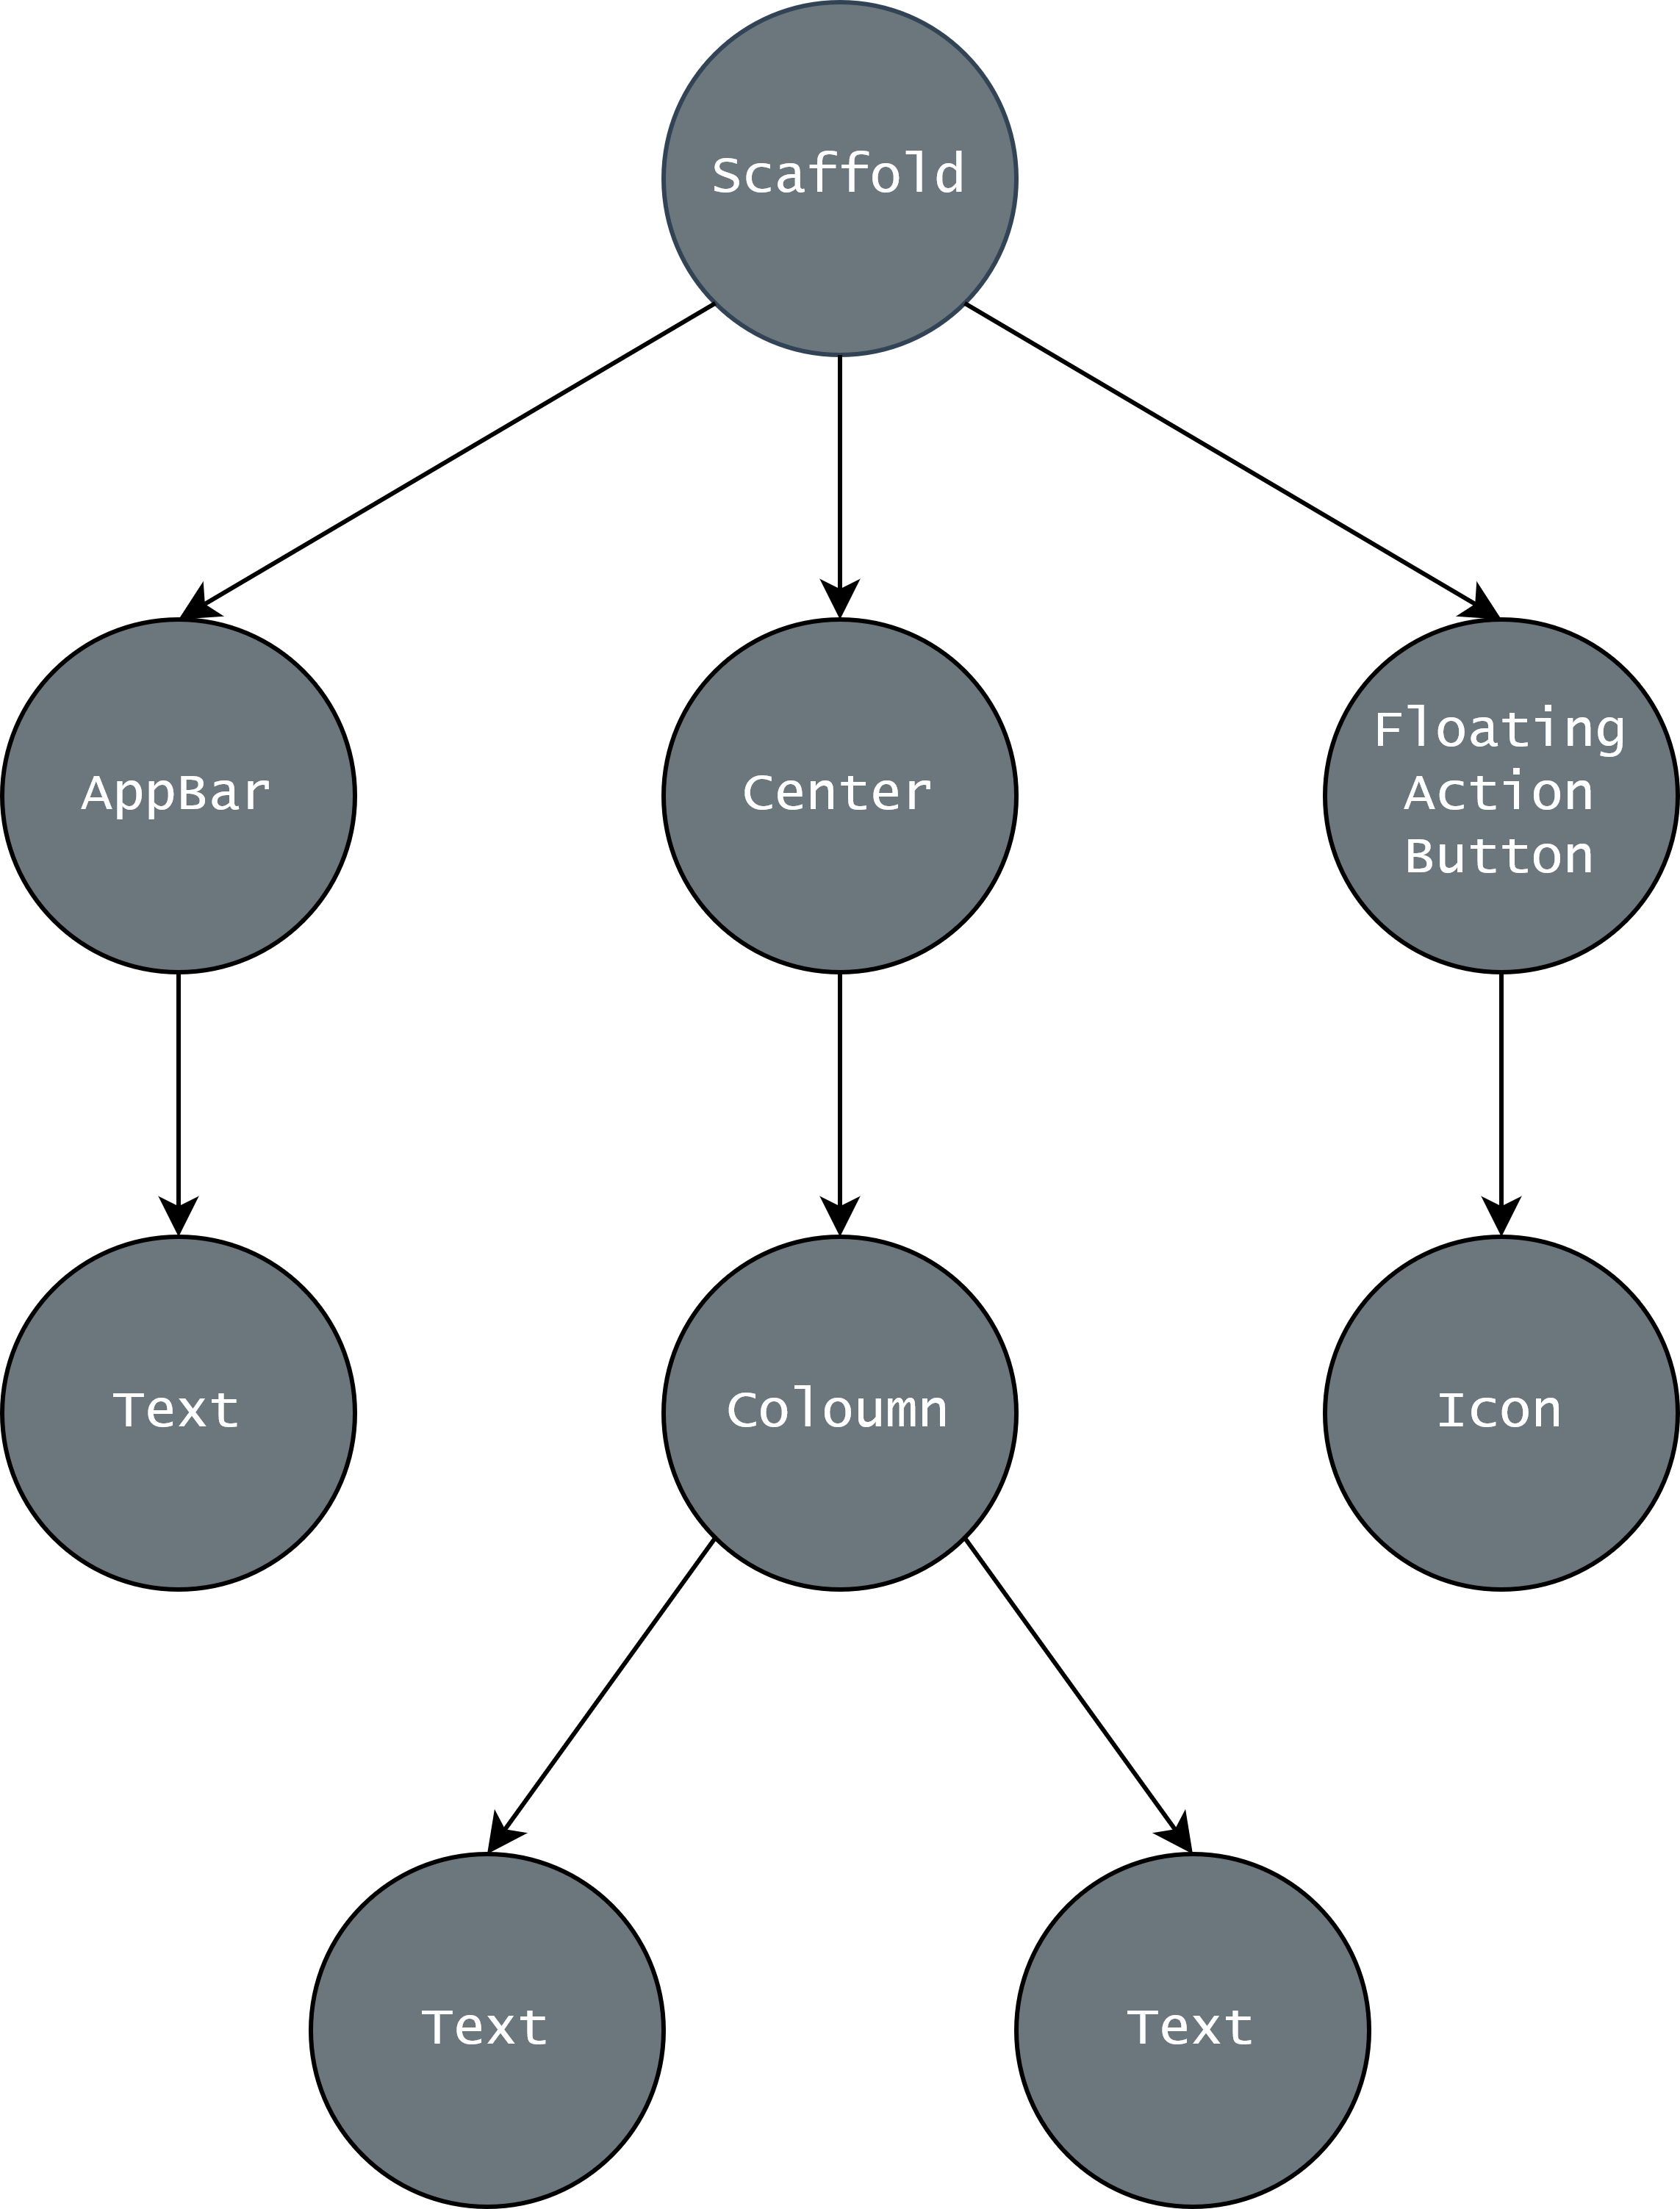
\includegraphics[height=8cm]{app_esempio_render_tree.png}\hspace{15mm}
    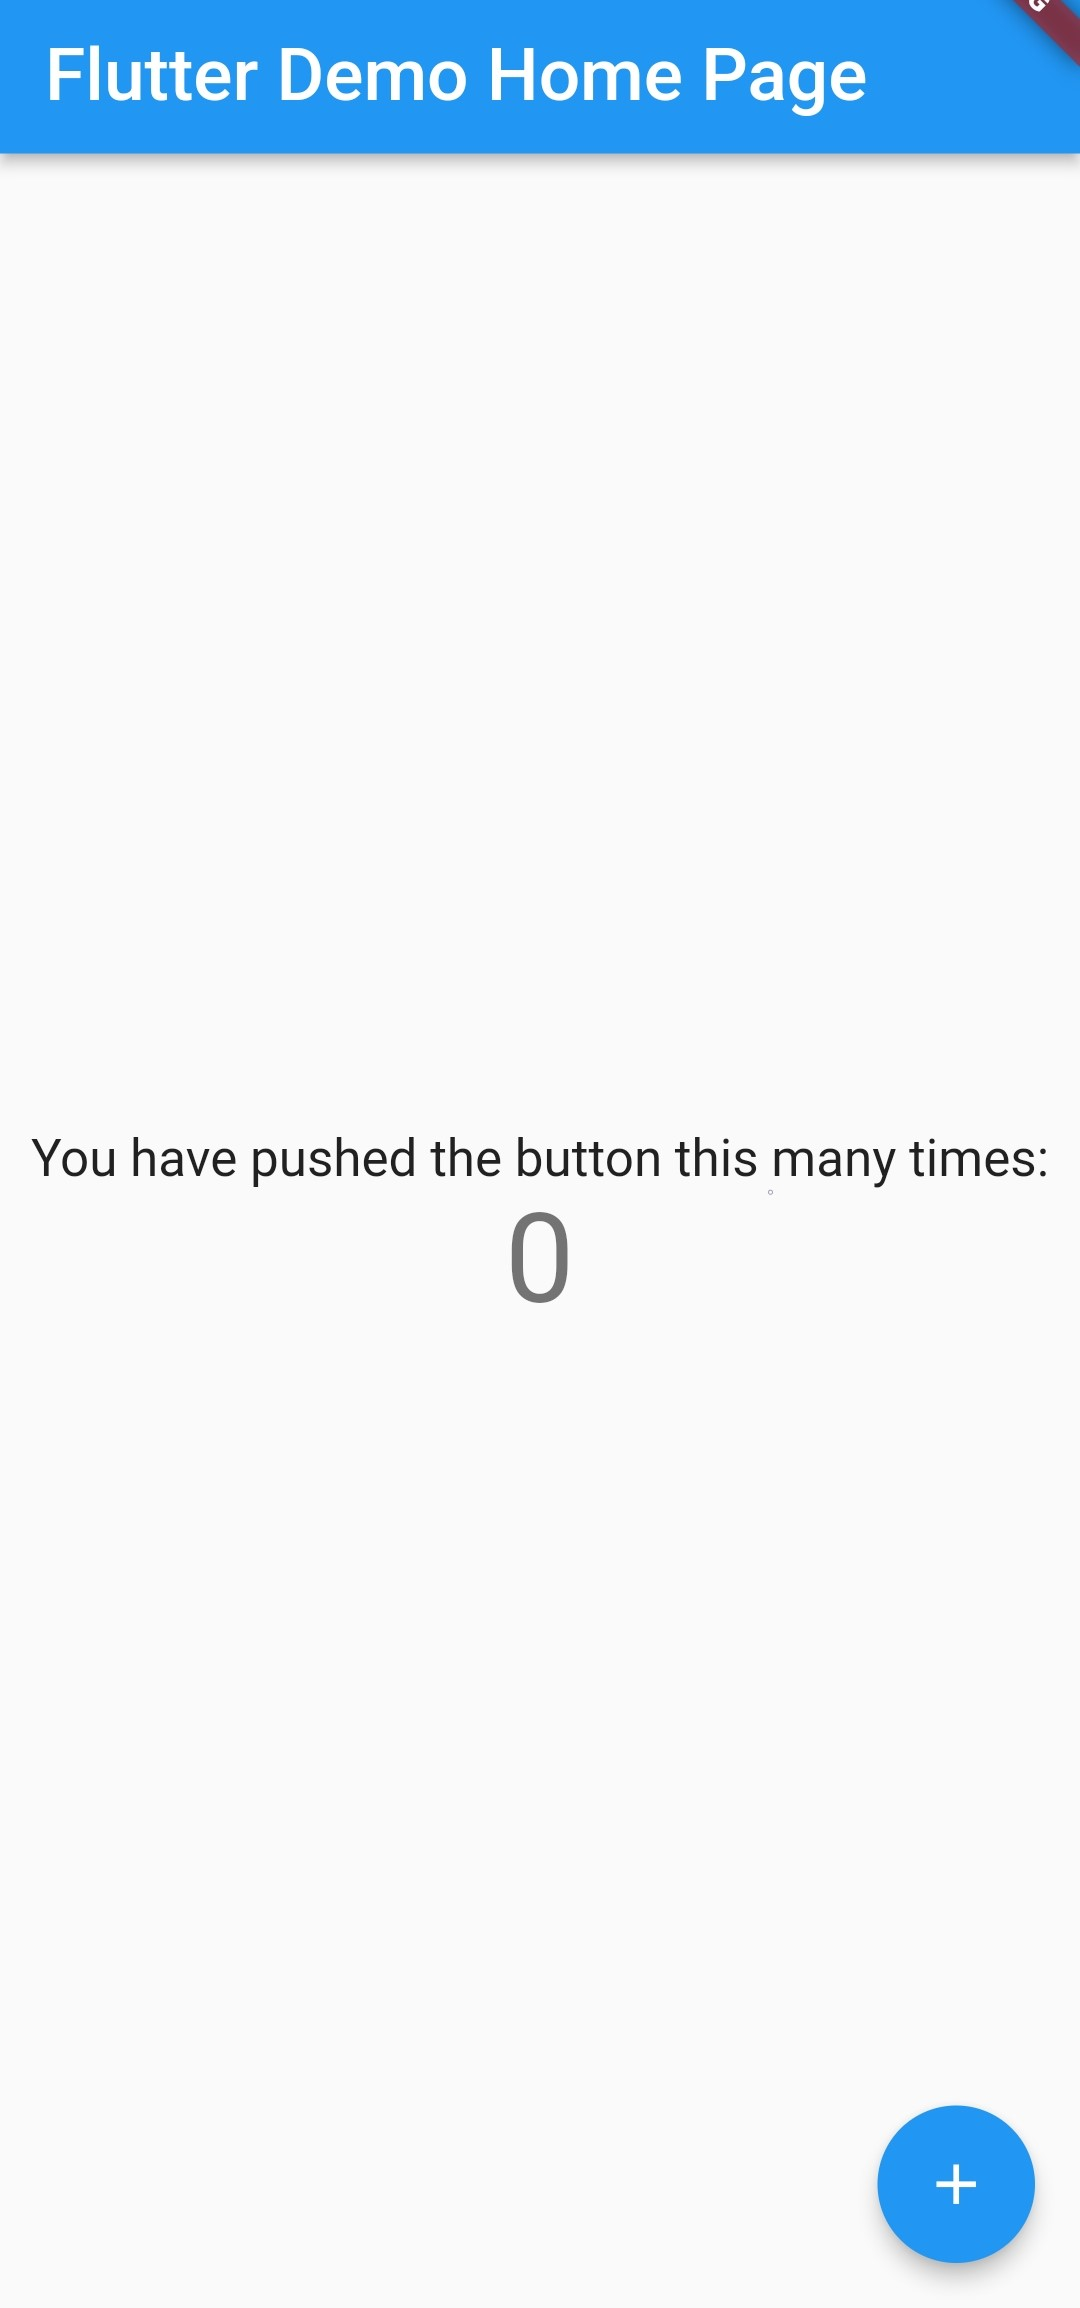
\includegraphics[height=8cm]{flutter_app_default.jpg}
    \caption[\textit{Widget tree} app esempio]{Il \textit{widget tree} dell'applicazione di esempio di Flutter e il suo risultato su Android}
\end{figure}

Per quanto riguarda le dimensioni delle varie componenti, Flutter ragiona come segue: i padri passano ai figli (dall'altro verso il basso nel \textit{widget tree}) dei \textit{"constraints"}, ovvero le dimensioni massime oltre le quali non possono cresce, e i figli passano quindi ai padri (dal basso verso l'alto nel \textit{widget tree}) le proprie dimensioni.\\
Il \textit{widget tree} è quello più importante da tenere a mente, e che più direttamente si interfaccia con il codice scritto dal programmatore. \\
Torniamo però alla figura \ref{fig:flutter-trees} per parlare brevemente degli altri due alberi: l'\textit{element tree} rappresenta gli elementi che, a differenza dei \textit{widget}, sono mutabili e vengono definiti come "un'istanza di un \textit{widget} in una particolare posizione dell'albero". Gli elementi sono responsabili di aggiornare l'interfaccia utente e fungono da ponte tra \verb+Widget+ e \verb+Render Object+.\\
Il \textit{render tree} rappresenta i \verb+Render Object+ e viene interpellato dal \textit{framework} per disegnare i componenti dell'interfaccia grafica. Una singola istanza di \verb+Render Object+ contiene tutte le informazioni riguardanti dimensioni, colori e logiche di \textit{layout} di un \verb+Widget+.\\
Abbiamo accennato che i \textit{widget} quando cambiano stato richiamano il proprio metodo \verb+build+ che provoca quindi una ricostruzione del \textit{widget} stesso. Questi \textit{widget} si chiamano "\textit{stateful}", e sono in diretta contrapposizione con quelli incapaci di modificarsi durante l'esecuzione, chiamati "\textit{stateless}". \\
Vediamo un esempio di \textit{stateful widget}:

\begin{lstlisting}[language=dart, label={lst:stateful_widget}, caption={Creazione \textit{stateless widget}}]
class MyApp extends StatelessWidget {
  //stateless widget che fa da radice per l'applicazione
  const MyApp({super.key});

  @override
  Widget build(BuildContext context) {
    return MaterialApp(
        home: const MyHomePage(title: 'Flutter Demo Home Page'),
    );
  }
}

class MyHomePage extends StatefulWidget {
  //qui passiamo allo stateful widget
  const MyHomePage({super.key, required this.title});
  final String title;

  @override
  //e qui creiamo lo stato vero e proprio
  State<MyHomePage> createState() => _MyHomePageState();
}


class _MyHomePageState extends State<MyHomePage> {
  int _counter = 0;

  void _incrementCounter() {
    //quando viene chiamata questa funzione viene
    //richiamato il metodo build, di fatto cambiando lo stato 
    //del widget e provocando un re-render dell'applicazione
    setState(() {
      _counter++;
    });
  }

  @override
  Widget build(BuildContext context) {}
}
\end{lstlisting}

Si nota immediatamente che l'uso degli \textit{stateful widget} provoca scrittura di codice ridondante e si è quindi deciso di arginare questo problema, aumentando al contempo la condivisione di codice tra i \textit{widget}, introducendo i Flutter Hooks (ispirati dagli \textit{hooks} di React).
Vediamo quindi la riscrittura del codice mostrato nel frammento \ref{lst:stateful_widget} opportunamente modificato usando un \verb+HookWidget+:

\begin{lstlisting}[language=dart, caption={Creazione \textit{hook widget}}]
class MyApp extends StatelessWidget {
  //stateless widget che fa da radice per l'applicazione
  const MyApp({super.key});

  @override
  Widget build(BuildContext context) {
    return MaterialApp(
        home: const MyHomePage(title: 'Flutter Demo Home Page'),
    );
  }
}

class MyHomePage extends HookWidget {
  //basta questa classe per fare tutti gli step
  //necessari al cambio di stato

  const MyHomePage({super.key, required this.title});
  final String title;

  Widget  build (BuildContext context){
    //_counter viene inizializzato a zero e reso
    //l'hook per il cambio di stato, quindi quando
    //il suo valore cambia viene provocato un rebuild
    final _counter = useState(0)

    return Scaffold(
      appBar: AppBar(),
      body: Center(),
      floatingActionButton: FloatingActionButton(
        //qui il valore di _counter cambia
        //provocando una rebuild
        onPressed: () => _counter.value++,
      )
    )
  }
}
\end{lstlisting}

\section{Method Channels}
I \textit{method channel} nascono per uno scopo: utilizzare codice nativo tramite Flutter, ad esempio per chiamare \api{} \textit{platform-specific} in Kotlin o Java per Android, in Swift per iOS o in C++ per Windows.\\
Flutter non usa queste funzionalità tramite generazione di codice e preferisce un approccio basato sullo scambio di messaggi. Vediamone quindi un esempio per ottenere, tramite Java, il valore di carica della batteria di un dispositivo Android.\\
Per prima cosa è necessario agire sull'Android \textit{manifest} inserendo il nome dell'applicazione di Flutter, in questo caso \verb+batterylevel+ (l'applicazione si può creare con il comando: \verb+flutter create nome_applicazione+).

\begin{lstlisting}[language=XML, firstnumber=1,caption={Android \textit{manifest}}]
<manifest xmlns:android="http://schemas.android.com/apk/res/android"
  package="com.example.batterylevel">
\end{lstlisting}

A questo punto si vanno a costruire gli "agganci" per il \textit{method channel} in codice nativo, in questo caso quindi nell'attività principale di Java:

\begin{lstlisting}[language=Java, firstnumber=1,caption={Java \textit{main activity}}]
public class MainActivity extends FlutterActivity {
  //"samples.flutter.dev/battery" e' il nome del method channel
  //come definito in main.dart
  private static final String CHANNEL = "samples.flutter.dev/battery";

  @Override
  public void configureFlutterEngine(@NonNull FlutterEngine flutterEngine) {
      super.configureFlutterEngine(flutterEngine);
      new MethodChannel(flutterEngine.getDartExecutor()
                                     .getBinaryMessenger(), CHANNEL)
              .setMethodCallHandler(
                      (call, result) -> {
                          //Questo e' il metodo invocato nel main
                          //sfruttiamo "getBatteryLevel" per invocarlo
                          if (call.method.equals("getBatteryLevel")) {
                              //il metodo vero e proprio in Java
                              int batteryLevel = getBatteryLevel();
                              if (batteryLevel != -1) {
                                  result.success(batteryLevel);
                              } else {
                                  result.error("UNAVAILABLE", 
                                  "Battery level not available.", null);
                              }
                          } else {
                              result.notImplemented();
                          }
                      }
              );
  }

  private int getBatteryLevel() {
    //metodo che ritorna il valore di batteria del dispositivo
  }
\end{lstlisting}

Infine ci occupiamo di lanciare il messaggio da Flutter invocando il metodo:

\begin{lstlisting}[language=dart, firstnumber=1,caption={Dart \textit{main}}]
class MyHomePage extends HookWidget {
const MyHomePage({super.key});
//creo e definisco il method channel
static const platform = MethodChannel('samples.flutter.dev/battery');

  @override
  Widget build(BuildContext context) {
    var batteryLevel = useState('Unknown battery level.');

    return Material(
      child: Center(
        child: Column(
          mainAxisAlignment: MainAxisAlignment.spaceEvenly,
          children: [
            ElevatedButton(
              onPressed: () async {
                try {
                  //qui avviene l'effettiva invocazione del
                  // method channel che provoca una chiamata in Java
                  final int result =
                      await platform.invokeMethod('getBatteryLevel');
                  batteryLevel.value = 'Battery level at $result % .';
                } on PlatformException catch (e) {
                  batteryLevel.value =
                      "Failed to get battery level: '${e.message}'.";
                }
              },
              child: const Text('Get Battery Level'),
            ),
            Text(batteryLevel.value),
          ],
        ),
      ),
    );
  }
}
\end{lstlisting}

\end{appendices}
